\documentclass[11pt,a4paper]{article}
\usepackage[margin=1in]{geometry}
\usepackage{amsmath,amssymb,amsthm}
\usepackage{graphicx}
\usepackage{listings}
\usepackage{xcolor}
\usepackage{hyperref}
\usepackage{booktabs}
\usepackage{enumitem}
\usepackage{tikz}
\usetikzlibrary{shapes,arrows,positioning,fit,backgrounds}
\usepackage{float}
\usepackage{fancyhdr}
\usepackage{titlesec}

% Code listing style
\lstset{
    basicstyle=\ttfamily\small,
    breaklines=true,
    frame=single,
    backgroundcolor=\color{gray!10},
    keywordstyle=\color{blue},
    commentstyle=\color{green!60!black},
    stringstyle=\color{orange},
    numbers=left,
    numberstyle=\tiny\color{gray},
    numbersep=5pt
}

\pagestyle{fancy}
\fancyhf{}
\rhead{Backtest V2 Architecture}
\lhead{BetterSys}
\rfoot{Page \thepage}

\title{\textbf{Backtest V2: A Production-Grade HFT Backtesting Framework}\\[0.5em]
\large Architectural Exposition and Technical Deep-Dive}
\author{BetterSys Technical Documentation}
\date{January 2026}

\begin{document}

\maketitle

\begin{abstract}
This document provides a comprehensive architectural exposition of the \texttt{backtest\_v2} module within the BetterSys trading system. The module comprises approximately 106,000 lines of Rust code across 107 source files, implementing a production-grade, HFT-capable backtesting framework for Polymarket prediction markets. We examine the core design principles, component architecture, data flow, invariant enforcement mechanisms, and the trust/certification pipeline that enables production-deployable backtesting results. The system is specifically designed for 15-minute Up/Down binary outcome markets with sub-millisecond latency modeling and strict determinism guarantees.
\end{abstract}

\tableofcontents
\newpage

%==============================================================================
\section{Introduction and Design Philosophy}
%==============================================================================

\subsection{Motivation}
The \texttt{backtest\_v2} module was developed to address the fundamental challenges in HFT backtesting: preventing look-ahead bias, ensuring deterministic reproducibility, providing realistic execution simulation, and producing auditable results that can be trusted for production deployment decisions.

Traditional backtesting systems suffer from several critical flaws:
\begin{itemize}
    \item \textbf{Look-ahead bias}: Strategy logic accidentally uses future data
    \item \textbf{Unrealistic fills}: Optimistic maker fill assumptions inflate performance
    \item \textbf{Non-determinism}: Results vary across runs due to floating-point or concurrency
    \item \textbf{Unauditable outputs}: No cryptographic proof of what code/data produced results
\end{itemize}

\subsection{Core Design Principles}

The system is built on five foundational principles:

\begin{enumerate}
    \item \textbf{Hermetic Execution}: Strategy code is sandboxed and cannot access wall-clock time, filesystem, network, or environment variables. All time comes from the simulation clock.
    
    \item \textbf{Visibility Enforcement}: Events have both \texttt{source\_time} (when they occurred) and \texttt{arrival\_time} (when the system observes them). Strategy decisions can only use events where \texttt{arrival\_time $\leq$ decision\_time}.
    
    \item \textbf{Double-Entry Accounting}: All economic state changes (fills, fees, settlements) must flow through a balanced ledger where debits equal credits. Direct portfolio mutation is forbidden in production mode.
    
    \item \textbf{Deterministic Fingerprinting}: Every run produces a cryptographic fingerprint that changes if and only if observable behavior changes, enabling reproducibility verification.
    
    \item \textbf{Production-by-Default}: The default configuration is production-grade with all invariants enforced. Non-production modes require explicit opt-in.
\end{enumerate}

%==============================================================================
\section{System Architecture Overview}
%==============================================================================

\subsection{High-Level Component Diagram}

The system is organized into several interconnected subsystems:

\begin{figure}[H]
\centering
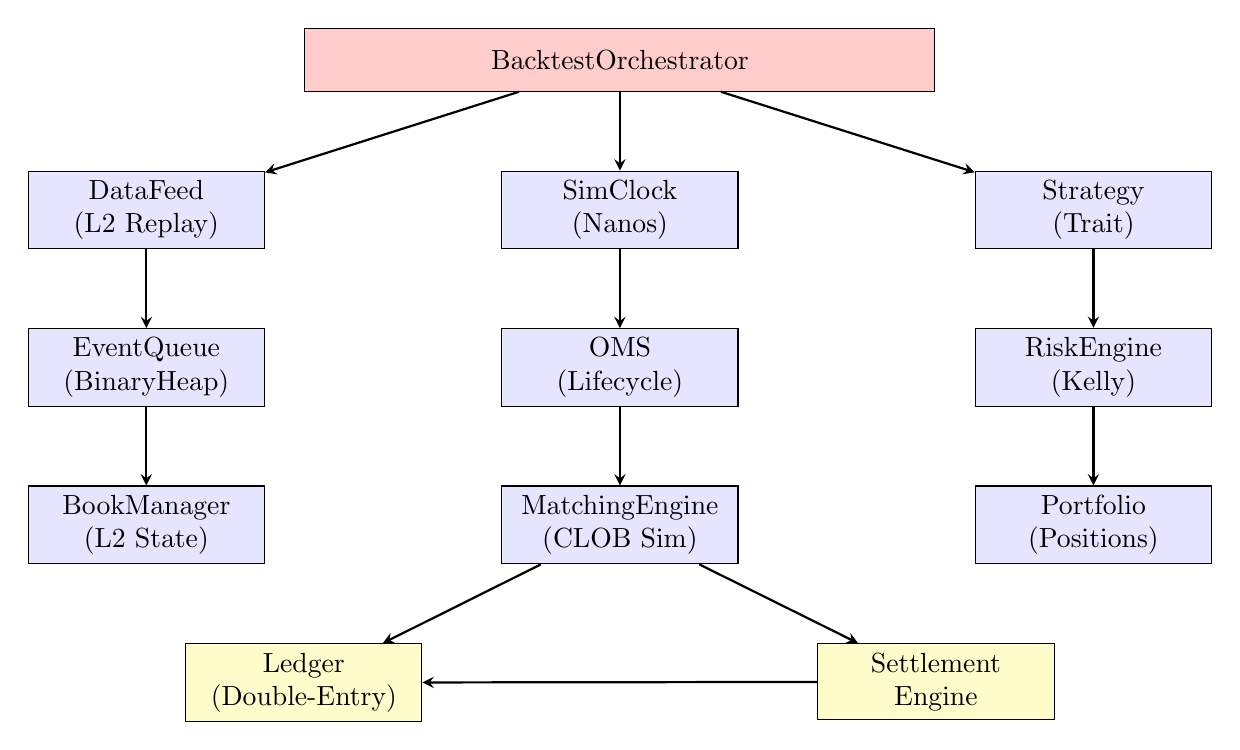
\begin{tikzpicture}[
    node distance=1.2cm,
    box/.style={rectangle, draw, fill=blue!10, minimum width=3cm, minimum height=0.8cm, align=center},
    smallbox/.style={rectangle, draw, fill=green!10, minimum width=2.2cm, minimum height=0.6cm, align=center, font=\small},
    arrow/.style={->, >=stealth, thick}
]

% Top level - Orchestrator
\node[box, fill=red!20, minimum width=8cm] (orch) {BacktestOrchestrator};

% Second level
\node[box, below left=1cm and 0.5cm of orch] (feed) {DataFeed\\(L2 Replay)};
\node[box, below=1cm of orch] (clock) {SimClock\\(Nanos)};
\node[box, below right=1cm and 0.5cm of orch] (strategy) {Strategy\\(Trait)};

% Third level
\node[box, below=1cm of feed] (queue) {EventQueue\\(BinaryHeap)};
\node[box, below=1cm of clock] (oms) {OMS\\(Lifecycle)};
\node[box, below=1cm of strategy] (risk) {RiskEngine\\(Kelly)};

% Fourth level
\node[box, below=1cm of queue] (book) {BookManager\\(L2 State)};
\node[box, below=1cm of oms] (matching) {MatchingEngine\\(CLOB Sim)};
\node[box, below=1cm of risk] (portfolio) {Portfolio\\(Positions)};

% Fifth level - Ledger and Settlement
\node[box, fill=yellow!20, below left=1cm and 1cm of matching] (ledger) {Ledger\\(Double-Entry)};
\node[box, fill=yellow!20, below right=1cm and 1cm of matching] (settlement) {Settlement\\Engine};

% Arrows
\draw[arrow] (orch) -- (feed);
\draw[arrow] (orch) -- (clock);
\draw[arrow] (orch) -- (strategy);
\draw[arrow] (feed) -- (queue);
\draw[arrow] (clock) -- (oms);
\draw[arrow] (strategy) -- (risk);
\draw[arrow] (queue) -- (book);
\draw[arrow] (oms) -- (matching);
\draw[arrow] (risk) -- (portfolio);
\draw[arrow] (matching) -- (ledger);
\draw[arrow] (matching) -- (settlement);
\draw[arrow] (settlement) -- (ledger);

\end{tikzpicture}
\caption{High-level component architecture of backtest\_v2}
\end{figure}

\subsection{File Organization}

The module contains 107 Rust source files organized by responsibility:

\begin{table}[H]
\centering
\begin{tabular}{lrl}
\toprule
\textbf{Category} & \textbf{Files} & \textbf{Purpose} \\
\midrule
Core Engine & 15 & Orchestrator, clock, events, queue \\
Order Management & 8 & OMS, matching, queue model, maker gate \\
Book Management & 6 & L2 state, deltas, snapshots, recording \\
Accounting & 5 & Ledger, portfolio, strict accounting \\
Settlement & 8 & 15M window, oracle, reference mapping \\
Invariants & 6 & Enforcer, visibility, integrity, validation \\
Fingerprinting & 4 & Run hash, reproducibility, certification \\
Metrics & 8 & Equity curve, window PnL, honesty \\
Oracle (submodule) & 9 & Chainlink, storage, backfill, diagnostics \\
Testing & 25 & Unit and integration test modules \\
\bottomrule
\end{tabular}
\caption{Source file organization by functional category}
\end{table}

%==============================================================================
\section{Core Engine Components}
%==============================================================================

\subsection{BacktestOrchestrator}

The \texttt{BacktestOrchestrator} (file: \texttt{orchestrator.rs}, $\sim$5,700 lines) is the central coordinator that:

\begin{itemize}
    \item Owns the simulation clock and drives the event loop
    \item Enforces determinism by controlling all sources of non-determinism
    \item Automatically determines the \textbf{Operating Mode} based on data quality
    \item Validates production-grade requirements at startup
    \item Produces the final \texttt{BacktestResults} with trust classification
\end{itemize}

\subsubsection{Operating Modes}

The system supports three operating modes, determined automatically:

\begin{lstlisting}[language=Rust, caption=Operating Mode Classification]
pub enum BacktestOperatingMode {
    TakerOnly,       // Maker fills disabled, aggressive only
    ResearchGrade,   // Indicative results, not production
    ProductionGrade, // Full fidelity, all claims valid
}
\end{lstlisting}

The mode is determined by:
\begin{enumerate}
    \item Data contract classification (FullIncremental required for Production)
    \item Maker fill model (ExplicitQueue required for Production)
    \item Strict mode and invariant enforcement settings
\end{enumerate}

\subsection{SimClock and Time Semantics}

Time is measured in nanoseconds (\texttt{Nanos = i64}) with three distinct timestamps per event:

\begin{itemize}
    \item \texttt{source\_time}: When the event occurred at the source (may be untrusted)
    \item \texttt{arrival\_time}: When the simulation "sees" the event
    \item \texttt{decision\_time}: Current clock time when strategy is invoked
\end{itemize}

\textbf{Hard Invariant}: Strategy logic may only access state from events where $\texttt{arrival\_time} \leq \texttt{decision\_time}$.

\subsection{EventQueue}

The \texttt{EventQueue} (\texttt{queue.rs}) implements a deterministic priority queue using a binary heap with composite ordering:

\begin{equation}
\text{Order} = (\texttt{time}, \texttt{priority}, \texttt{source}, \texttt{seq})
\end{equation}

where \texttt{priority} ensures system events (halts, resolutions) are processed before market data, which is processed before order events.

%==============================================================================
\section{Event Model and Data Structures}
%==============================================================================

\subsection{Canonical Event Types}

The \texttt{events.rs} module defines the canonical event types:

\begin{lstlisting}[language=Rust, caption=Core Event Types]
pub enum Event {
    L2BookSnapshot { token_id, bids, asks, exchange_seq },
    L2Delta { token_id, bid_updates, ask_updates, exchange_seq },
    L2BookDelta { token_id, side, price, new_size, seq_hash },
    TradePrint { token_id, price, size, aggressor_side, trade_id },
    OrderAck { order_id, client_order_id, exchange_time },
    OrderReject { order_id, client_order_id, reason },
    Fill { order_id, price, size, is_maker, leaves_qty, fee, fill_id },
    CancelAck { order_id, cancelled_qty },
    MarketStatusChange { token_id, new_status, reason },
    ResolutionEvent { token_id, resolution },
    Signal { signal_id, signal_type, market_slug, confidence, details },
    Timer { timer_id, payload },
}
\end{lstlisting}

\subsection{TimestampedEvent Ordering}

Events are wrapped in \texttt{TimestampedEvent} which implements deterministic ordering:

\begin{lstlisting}[language=Rust, caption=Deterministic Event Ordering]
impl Ord for TimestampedEvent {
    fn cmp(&self, other: &Self) -> Ordering {
        self.time.cmp(&other.time)
            .then_with(|| self.event.priority().cmp(&other.event.priority()))
            .then_with(|| self.source.cmp(&other.source))
            .then_with(|| self.seq.cmp(&other.seq))
    }
}
\end{lstlisting}

%==============================================================================
\section{Order Management System}
%==============================================================================

\subsection{OMS State Machine}

The Order Management System (\texttt{oms.rs}) implements a rigorous state machine for order lifecycle:

\begin{figure}[H]
\centering
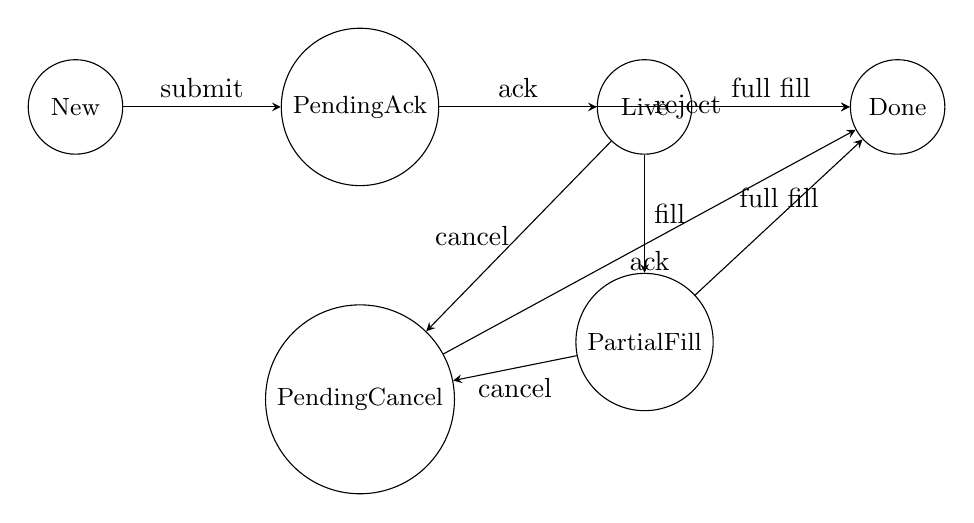
\begin{tikzpicture}[
    state/.style={circle, draw, minimum size=1.2cm, font=\small},
    arrow/.style={->, >=stealth}
]
\node[state] (new) {New};
\node[state, right=2cm of new] (pending) {Pending\\Ack};
\node[state, right=2cm of pending] (live) {Live};
\node[state, below=1.5cm of live] (partial) {Partial\\Fill};
\node[state, below=1.5cm of pending] (cancel) {Pending\\Cancel};
\node[state, right=2cm of live] (done) {Done};

\draw[arrow] (new) -- node[above] {submit} (pending);
\draw[arrow] (pending) -- node[above] {ack} (live);
\draw[arrow] (pending) -- node[right] {reject} (done);
\draw[arrow] (live) -- node[right] {fill} (partial);
\draw[arrow] (live) -- node[above] {full fill} (done);
\draw[arrow] (partial) -- node[above] {full fill} (done);
\draw[arrow] (live) -- node[left] {cancel} (cancel);
\draw[arrow] (partial) -- node[below] {cancel} (cancel);
\draw[arrow] (cancel) -- node[below] {ack} (done);
\end{tikzpicture}
\caption{OMS state machine transitions}
\end{figure}

\subsection{OMS Parity Modes}

The system supports different OMS validation levels:

\begin{itemize}
    \item \textbf{Full}: All state transitions are validated; invalid transitions abort
    \item \textbf{Relaxed}: Warnings on invalid transitions; continues execution
    \item \textbf{Disabled}: No validation (testing only, marks results untrusted)
\end{itemize}

\subsection{Queue Position Model}

The \texttt{QueuePositionModel} (\texttt{queue\_model.rs}) tracks FIFO queue positions for maker orders:

\begin{itemize}
    \item Tracks orders by price level in FIFO order
    \item Processes L2 deltas to update queue positions
    \item Handles cancel-fill race conditions
    \item Estimates fill probability based on queue position
\end{itemize}

\begin{lstlisting}[language=Rust, caption=Queue Position Tracking]
pub struct QueuePosition {
    pub order_id: OrderId,
    pub position: usize,      // 0 = front of queue
    pub size_ahead: Size,     // Volume ahead in queue
    pub our_size: Size,
    pub joined_at: Nanos,
}
\end{lstlisting}

\subsection{Maker Fill Gate}

The \texttt{MakerFillGate} (\texttt{maker\_fill\_gate.rs}) validates every maker fill candidate:

\begin{enumerate}
    \item Verify queue position was consumed by observed trade prints
    \item Check cancel-fill race timing
    \item Validate price level existed in the order book
    \item Reject fills without sufficient proof
\end{enumerate}

Only fills that pass all validations are admitted to the ledger.

%==============================================================================
\section{Matching Engine Simulation}
%==============================================================================

\subsection{Limit Order Book Simulator}

The \texttt{MatchingEngine} (\texttt{matching.rs}) provides full CLOB simulation:

\begin{itemize}
    \item FIFO price-time priority matching
    \item Partial fills with leaves quantity tracking
    \item Self-trade prevention (STP) with multiple modes
    \item Post-only order rejection when would cross
    \item Configurable maker/taker fees
\end{itemize}

\subsection{Price Representation}

Prices are internally represented as integer ticks for deterministic matching:

\begin{lstlisting}[language=Rust, caption=Price Tick Conversion]
pub const DEFAULT_TICK_SIZE: f64 = 0.01;  // Polymarket cent ticks

pub fn price_to_ticks(price: f64, tick_size: f64) -> PriceTicks {
    ((price / tick_size).round() as u32).clamp(1, 99)
}
\end{lstlisting}

\subsection{Fee Configuration}

\begin{lstlisting}[language=Rust, caption=Fee Configuration]
pub struct FeeConfig {
    pub maker_fee_rate: f64,   // Negative = rebate
    pub taker_fee_rate: f64,   // Typically 10bps for Polymarket
}
\end{lstlisting}

%==============================================================================
\section{Double-Entry Ledger System}
%==============================================================================

\subsection{Design Philosophy}

The ledger system (\texttt{ledger.rs}, $\sim$800 lines) implements classical double-entry accounting:

\begin{quote}
\textit{Every economic state change must be recorded as balanced entries where total debits equal total credits.}
\end{quote}

\subsection{Account Types}

\begin{lstlisting}[language=Rust, caption=Ledger Account Types]
pub enum LedgerAccount {
    Cash,                                    // USDC balance
    CostBasis { market_id, outcome },        // Position cost basis
    FeesPaid,                                // Accumulated fees
    Capital,                                 // Contributed equity
    RealizedPnL,                             // Trading profits/losses
    SettlementReceivable { market_id },      // Amounts owed to us
    SettlementPayable { market_id },         // Amounts we owe
}
\end{lstlisting}

\subsection{Fixed-Point Arithmetic}

To avoid floating-point errors, all amounts use fixed-point representation:

\begin{lstlisting}[language=Rust, caption=Fixed-Point Amount]
pub type Amount = i128;
pub const AMOUNT_SCALE: i128 = 100_000_000;  // 8 decimal places

pub fn to_amount(value: f64) -> Amount {
    (value * AMOUNT_SCALE as f64).round() as Amount
}
\end{lstlisting}

\subsection{Continuous Accounting Invariants}

The ledger enforces four invariants after every entry:

\begin{enumerate}
    \item \textbf{Cash non-negativity}: $\text{Cash} \geq 0$ (unless margin enabled)
    \item \textbf{Position non-negativity}: $\text{Position} \geq 0$ (unless shorting enabled)
    \item \textbf{Balance conservation}: $\sum \text{debits} = \sum \text{credits}$
    \item \textbf{No orphaned cost basis}: If position $= 0$, then cost basis $= 0$
\end{enumerate}

\subsection{Strict Accounting Mode}

When \texttt{strict\_accounting = true} (required for production-grade):

\begin{itemize}
    \item Direct portfolio mutations are forbidden
    \item All fills, fees, settlements flow through the ledger
    \item First invariant violation aborts immediately with causal trace
    \item Portfolio positions become derived-only from ledger state
\end{itemize}

%==============================================================================
\section{Settlement Engine}
%==============================================================================

\subsection{15-Minute Up/Down Market Settlement}

The settlement engine (\texttt{settlement.rs}) implements exact contract semantics for Polymarket 15-minute Up/Down markets:

\begin{itemize}
    \item Window duration: 15 minutes (900 seconds)
    \item Reference price: Binance spot mid-price
    \item Up wins if: $\text{end\_price} > \text{start\_price}$
    \item Down wins if: $\text{end\_price} \leq \text{start\_price}$ (tie goes to Down)
\end{itemize}

\subsection{Settlement Specification}

\begin{lstlisting}[language=Rust, caption=Settlement Specification]
pub struct SettlementSpec {
    pub market_type: String,
    pub window_duration_ns: Nanos,
    pub window_start_rule: WindowStartRule,
    pub reference_price_rule: ReferencePriceRule,
    pub rounding_rule: RoundingRule,
    pub tie_rule: TieRule,
    pub outcome_knowable_rule: OutcomeKnowableRule,
}
\end{lstlisting}

\subsection{Visibility Semantics for Settlement}

\textbf{Critical}: The outcome is NOT knowable at the cutoff time. It becomes knowable only when the reference price event has \textbf{arrived} (visibility enforcement):

\begin{lstlisting}[language=Rust, caption=Outcome Knowability]
match self.spec.outcome_knowable_rule {
    OutcomeKnowableRule::OnReferenceArrival => {
        decision_time >= end_price_arrival_ns
    }
    OutcomeKnowableRule::DelayFromCutoff { delay_ns } => {
        decision_time >= window_end_ns + delay_ns
    }
}
\end{lstlisting}

\subsection{Oracle Integration}

The \texttt{oracle/} submodule provides Chainlink integration for production settlement:

\begin{itemize}
    \item \texttt{ChainlinkIngestor}: Fetches rounds from RPC
    \item \texttt{OracleRoundStorage}: SQLite persistence with arrival-time
    \item \texttt{ChainlinkSettlementSource}: Settlement reference provider
    \item \texttt{BasisDiagnostics}: Tracks Chainlink vs Binance basis
\end{itemize}

%==============================================================================
\section{Invariant Enforcement Framework}
%==============================================================================

\subsection{Mandatory Invariant Checking}

The \texttt{InvariantEnforcer} (\texttt{invariants.rs}, $\sim$1,700 lines) promotes invariant checking from optional debugging to a mandatory structural requirement.

\subsection{Invariant Categories}

\begin{table}[H]
\centering
\begin{tabular}{ll}
\toprule
\textbf{Category} & \textbf{Checks} \\
\midrule
Time & Decision time monotonicity, visibility semantics, event ordering \\
Book & Crossed book detection, price validity, size positivity \\
OMS & Order lifecycle correctness, illegal state transitions \\
Fills & Plausibility checks, overfill prevention, price validity \\
Accounting & Double-entry balance, cash non-negativity, equity identity \\
\bottomrule
\end{tabular}
\caption{Invariant categories and their checks}
\end{table}

\subsection{Enforcement Modes}

\begin{lstlisting}[language=Rust, caption=Invariant Modes]
pub enum InvariantMode {
    Off,   // Disabled (INVALID for production)
    Soft,  // Log + count violations, continue
    Hard,  // Abort on first violation with causal dump
}
\end{lstlisting}

\subsection{Causal Dump on Abort}

When an invariant violation occurs in Hard mode, the system produces a deterministic \texttt{CausalDump}:

\begin{itemize}
    \item The specific violation that triggered the abort
    \item Last N events leading to the violation
    \item Last N OMS state transitions
    \item Last N ledger entries
    \item State snapshot (book, cash, positions)
    \item Run fingerprint at abort time
\end{itemize}

%==============================================================================
\section{Visibility and Look-Ahead Prevention}
%==============================================================================

\subsection{SimArrivalPolicy}

The \texttt{visibility.rs} module implements look-ahead prevention:

\begin{lstlisting}[language=Rust, caption=Arrival Time Policies]
pub enum SimArrivalPolicy {
    RecordedArrival,    // Use historical arrival_time (best)
    SimulatedLatency {  // Derive from source_time + latency
        market_data_latency: LatencyDistribution,
        internal_event_latency: LatencyDistribution,
        seed: u64,
    },
    Unusable,           // Blocks production-grade claims
}
\end{lstlisting}

\subsection{VisibilityWatermark}

The \texttt{VisibilityWatermark} tracks what data is visible:

\begin{lstlisting}[language=Rust, caption=Visibility Enforcement]
pub struct VisibilityWatermark {
    decision_time: Nanos,
    latest_applied_arrival: Nanos,
    events_applied: u64,
    violations: Vec<VisibilityViolation>,
}

// Invariant: latest_applied_arrival <= decision_time
\end{lstlisting}

\subsection{DecisionProof}

Every strategy decision produces a \texttt{DecisionProof} documenting:

\begin{itemize}
    \item Decision ID and timestamp
    \item All input events that affected state since last decision
    \item Proof hash for quick comparison
\end{itemize}

%==============================================================================
\section{Hermetic Strategy Execution}
%==============================================================================

\subsection{Compile-Time Enforcement}

The \texttt{hermetic.rs} module enforces strategy sandboxing:

\begin{lstlisting}[language=Rust, caption=Forbidden API Patterns]
pub const FORBIDDEN_API_PATTERNS: &[&str] = &[
    "std::time::SystemTime",
    "std::time::Instant",
    "tokio::time::Instant",
    "chrono::Utc::now",
    "chrono::Local::now",
    "std::env::var",
    "std::fs::",
    "tokio::net::",
    "std::thread::spawn",
];
\end{lstlisting}

\subsection{Runtime Guards}

Additional runtime guards prevent:
\begin{itemize}
    \item Wall-clock access
    \item Environment variable reads
    \item Filesystem I/O
    \item Network I/O
    \item Thread/task spawning
\end{itemize}

\subsection{HermeticConfig}

\begin{lstlisting}[language=Rust, caption=Hermetic Configuration]
pub struct HermeticConfig {
    pub enabled: bool,
    pub require_decision_proofs: bool,
    pub abort_on_violation: bool,
    pub track_violations: bool,
}
\end{lstlisting}

%==============================================================================
\section{Fingerprinting and Reproducibility}
%==============================================================================

\subsection{Run Fingerprint Structure}

The \texttt{RunFingerprint} (\texttt{fingerprint.rs}) provides cryptographic auditability:

\begin{equation}
\text{RunFingerprint} = H(\text{Version} \| \text{Strategy} \| \text{Code} \| \text{Config} \| \text{Dataset} \| \text{Seed} \| \text{Behavior})
\end{equation}

\subsection{Component Fingerprints}

\begin{itemize}
    \item \textbf{StrategyFingerprint}: Name, version, code hash
    \item \textbf{CodeFingerprint}: Crate version, git commit, build profile
    \item \textbf{ConfigFingerprint}: All behavior-affecting config
    \item \textbf{DatasetFingerprint}: Stream hashes, record counts, time ranges
    \item \textbf{SeedFingerprint}: Primary seed and derived sub-seeds
    \item \textbf{BehaviorFingerprint}: Rolling hash of all observable events
\end{itemize}

\subsection{Observable Behavior Events}

The behavior fingerprint captures (in deterministic order):
\begin{enumerate}
    \item Strategy decisions (DecisionProof hashes)
    \item Orders emitted (id, side, price, size, type, time)
    \item OMS outcomes (ack/reject/cancel ack)
    \item Fills (price, size, maker/taker flag, time)
    \item Fees posted
    \item Settlement events and outcomes
    \item Ledger postings
    \item Window PnL series
    \item Equity curve
\end{enumerate}

\subsection{Reproducibility Verification}

The \texttt{ReproducibilityCollector} (\texttt{reproducibility.rs}) enables cross-run verification:

\begin{lstlisting}[language=Rust, caption=Replay Verification]
pub struct ReplayVerificationResult {
    pub identical: bool,
    pub first_mismatch: Option<ReplayMismatch>,
    pub events_compared: u64,
    pub reference_hash: u64,
    pub replay_hash: u64,
}
\end{lstlisting}

%==============================================================================
\section{Trust Gate and Certification}
%==============================================================================

\subsection{TrustGate Evaluation}

The \texttt{TrustGate} (\texttt{trust\_gate.rs}) is the authoritative source for trust classification:

\begin{lstlisting}[language=Rust, caption=Trust Decision]
pub struct TrustDecision {
    pub level: TrustLevel,
    pub failures: Vec<TrustFailureReason>,
    pub evaluated_at: Nanos,
    pub fingerprint_hash: u64,
}

pub enum TrustLevel {
    Trusted,     // All requirements satisfied
    Untrusted,   // One or more critical failures
}
\end{lstlisting}

\subsection{Trust Requirements}

For \texttt{TrustLevel::Trusted}:
\begin{itemize}
    \item Production-grade mode enabled
    \item All invariants passed (Hard mode)
    \item Settlement used ExactSpec model
    \item Double-entry ledger enforced with no violations
    \item Data classification is FullIncremental
    \item Gate suite passed
    \item No sensitivity fragilities
    \item OMS parity is Full
    \item Hermetic strategy mode enabled
\end{itemize}

\subsection{Gate Suite}

The \texttt{GateSuite} (\texttt{gate\_suite.rs}) runs adversarial tests:

\begin{itemize}
    \item \textbf{DoNothingStrategy}: Verifies zero PnL when no trading
    \item \textbf{RandomTakerStrategy}: Tests execution under random load
    \item \textbf{SignalInverter}: Checks that inverted signals lose money
    \item \textbf{ZeroEdgeWrapper}: Verifies zero-edge strategies break even
\end{itemize}

%==============================================================================
\section{Metrics and Reporting}
%==============================================================================

\subsection{Equity Curve}

The \texttt{EquityRecorder} (\texttt{equity\_curve.rs}) produces a canonical equity curve:

\begin{itemize}
    \item Points recorded at economically meaningful times (fills, fees, settlements)
    \item Derived from ledger state (not portfolio)
    \item Deterministic and reproducible
    \item Final equity matches ledger computation
\end{itemize}

\subsection{Window PnL Series}

The \texttt{WindowAccountingEngine} (\texttt{window\_pnl.rs}) tracks per-15-minute window PnL:

\begin{lstlisting}[language=Rust, caption=Window PnL]
pub struct WindowPnL {
    pub window_id: WindowId,
    pub window_start: Nanos,
    pub window_end: Nanos,
    pub gross_pnl: Amount,
    pub fees: Amount,
    pub net_pnl: Amount,
    pub trade_count: u64,
}
\end{lstlisting}

\textbf{Invariant}: $\sum \text{window.net\_pnl} = \text{total net PnL}$

\subsection{Honesty Metrics}

The \texttt{HonestyMetrics} (\texttt{honesty.rs}) prevent misleading PnL screenshots:

\begin{itemize}
    \item Normalized returns per window
    \item Fee impact ratios
    \item Distribution statistics across windows
\end{itemize}

\subsection{Disclaimers Block}

The \texttt{DisclaimersBlock} (\texttt{disclaimers.rs}) generates programmatic caveats:

\begin{lstlisting}[language=Rust, caption=Disclaimer Structure]
pub struct Disclaimer {
    pub category: Category,
    pub severity: Severity,
    pub message: String,
    pub technical_detail: Option<String>,
}
\end{lstlisting}

%==============================================================================
\section{Data Contract and Readiness}
%==============================================================================

\subsection{Historical Data Contract}

The \texttt{HistoricalDataContract} (\texttt{data\_contract.rs}) declares dataset capabilities:

\begin{lstlisting}[language=Rust, caption=Data Contract]
pub struct HistoricalDataContract {
    pub venue: String,
    pub market: String,
    pub orderbook: OrderBookHistory,
    pub trades: TradeHistory,
    pub arrival_time: ArrivalTimeSemantics,
}
\end{lstlisting}

\subsection{Dataset Classification}

\begin{lstlisting}[language=Rust, caption=Dataset Classification]
pub enum DatasetClassification {
    FullIncremental,    // L2 deltas + trades + arrival times
    SnapshotOnly,       // Periodic snapshots, no deltas
    Incomplete,         // Missing critical data
}
\end{lstlisting}

\subsection{Readiness Classification}

\begin{lstlisting}[language=Rust, caption=Dataset Readiness]
pub enum DatasetReadiness {
    MakerViable,       // Supports queue modeling
    TakerOnly,         // Only aggressive execution valid
    NonRepresentative, // Results not trustworthy
}
\end{lstlisting}

%==============================================================================
\section{L2 Data Pipeline}
%==============================================================================

\subsection{L2 Delta Model}

The \texttt{l2\_delta.rs} module implements HFT-grade book reconstruction:

\begin{lstlisting}[language=Rust, caption=L2 Delta Event]
pub struct PolymarketL2Delta {
    pub asset: String,
    pub timestamp_ns: i64,
    pub side: BookSide,
    pub price: TickPriceLevel,
    pub new_size: u64,       // Size in shares (scaled)
    pub hash: Option<String>, // Exchange sequence hash
}
\end{lstlisting}

\subsection{Deterministic Book Reconstruction}

The \texttt{DeterministicBook} maintains book state with:
\begin{itemize}
    \item Sequence gap detection
    \item Crossed book validation
    \item Fingerprint tracking for reproducibility
\end{itemize}

\subsection{Trade Print Attribution}

The \texttt{TradePrintAttributionEngine} (\texttt{trade\_print\_attribution.rs}):
\begin{itemize}
    \item Tracks mid-price moves at horizons (100ms, 500ms, 1s, 5s)
    \item Computes adverse selection metrics
    \item Attributes fills to nearby trade prints
\end{itemize}

%==============================================================================
\section{Sensitivity Analysis}
%==============================================================================

\subsection{Fragility Detection}

The \texttt{SensitivityConfig} (\texttt{sensitivity.rs}) enables parameter sweeps:

\begin{lstlisting}[language=Rust, caption=Sensitivity Configuration]
pub struct SensitivityConfig {
    pub enabled: bool,
    pub latency_sweep: Option<LatencySweepConfig>,
    pub sampling_sweep: Option<SamplingSweepConfig>,
    pub execution_sweep: Option<ExecutionSweepConfig>,
}
\end{lstlisting}

\subsection{Fragility Flags}

\begin{lstlisting}[language=Rust, caption=Fragility Detection]
pub struct FragilityFlags {
    pub latency_fragile: bool,
    pub sampling_fragile: bool,
    pub execution_fragile: bool,
    pub requires_optimistic_assumptions: bool,
}
\end{lstlisting}

A strategy is marked fragile if small parameter changes cause large PnL swings.

%==============================================================================
\section{Artifact Storage and Publication}
%==============================================================================

\subsection{Run Artifact Structure}

The \texttt{RunArtifact} (\texttt{run\_artifact.rs}) is the complete output package:

\begin{lstlisting}[language=Rust, caption=Run Artifact]
pub struct RunArtifact {
    pub manifest: RunManifest,
    pub equity_curve: EquityCurve,
    pub window_pnl: WindowPnLSeries,
    pub distributions: RunDistributions,
    pub time_series: RunTimeSeries,
    pub fingerprint: RunFingerprint,
    pub trust_decision: TrustDecision,
    pub disclaimers: DisclaimersBlock,
}
\end{lstlisting}

\subsection{Artifact Store}

The \texttt{ArtifactStore} (\texttt{artifact\_store.rs}) provides persistent storage with:
\begin{itemize}
    \item Immutable artifact storage by run ID
    \item Listing and filtering capabilities
    \item Integrity verification on load
\end{itemize}

\subsection{Publication Gate}

The \texttt{PublicationGate} (\texttt{publication.rs}) controls what can be published:
\begin{itemize}
    \item Only \texttt{TrustLevel::Trusted} runs can be published
    \item Warns on untrusted publication attempts
    \item Enforces disclaimer inclusion
\end{itemize}

%==============================================================================
\section{Strategy Interface}
%==============================================================================

\subsection{Strategy Trait}

\begin{lstlisting}[language=Rust, caption=Strategy Trait]
pub trait Strategy: Send {
    fn on_book_update(&mut self, ctx: &mut StrategyContext, book: &BookSnapshot);
    fn on_trade(&mut self, ctx: &mut StrategyContext, trade: &TradePrint);
    fn on_timer(&mut self, ctx: &mut StrategyContext, timer: &TimerEvent);
    fn on_order_ack(&mut self, ctx: &mut StrategyContext, ack: &OrderAck);
    fn on_order_reject(&mut self, ctx: &mut StrategyContext, reject: &OrderReject);
    fn on_fill(&mut self, ctx: &mut StrategyContext, fill: &FillNotification);
    fn on_cancel_ack(&mut self, ctx: &mut StrategyContext, ack: &CancelAck);
    fn on_start(&mut self, ctx: &mut StrategyContext);
    fn on_stop(&mut self, ctx: &mut StrategyContext);
    fn name(&self) -> &str;
}
\end{lstlisting}

\subsection{OrderSender Interface}

The \texttt{OrderSender} trait abstracts order submission:

\begin{lstlisting}[language=Rust, caption=Order Sender Interface]
pub trait OrderSender: Send + Sync {
    fn send_order(&mut self, order: StrategyOrder) -> Result<OrderId, String>;
    fn send_cancel(&mut self, cancel: StrategyCancel) -> Result<(), String>;
    fn cancel_all(&mut self, token_id: &str) -> Result<usize, String>;
    fn get_position(&self, token_id: &str) -> Position;
    fn get_open_orders(&self) -> Vec<OpenOrder>;
    fn now(&self) -> Nanos;
    fn schedule_timer(&mut self, delay_ns: Nanos, payload: Option<String>) -> u64;
}
\end{lstlisting}

%==============================================================================
\section{Conclusion}
%==============================================================================

The \texttt{backtest\_v2} module represents a comprehensive solution to the challenges of HFT backtesting. Its key innovations include:

\begin{enumerate}
    \item \textbf{Production-by-Default}: The path of least resistance produces auditable, trustworthy results.
    
    \item \textbf{Multi-Layer Invariant Enforcement}: Time, book, OMS, fill, and accounting invariants catch errors at the earliest possible point.
    
    \item \textbf{Cryptographic Auditability}: Run fingerprints enable verification that specific code, config, and data produced specific results.
    
    \item \textbf{Realistic Execution Modeling}: Queue position tracking, cancel-fill races, and maker fill validation prevent optimistic bias.
    
    \item \textbf{Double-Entry Accounting}: Balanced ledger entries ensure economic consistency and catch accounting bugs.
    
    \item \textbf{Visibility Enforcement}: Strict arrival-time semantics prevent look-ahead bias.
    
    \item \textbf{Hermetic Strategy Execution}: Sandbox enforcement ensures strategies cannot accidentally access forbidden state.
\end{enumerate}

The system is designed for Polymarket 15-minute Up/Down markets but the architecture generalizes to any CLOB-based venue with binary outcomes and deterministic settlement rules.

\subsection{Scale and Complexity}

\begin{itemize}
    \item \textbf{Total Lines}: $\sim$106,000 lines of Rust
    \item \textbf{Source Files}: 107 modules
    \item \textbf{Test Files}: 25 test modules
    \item \textbf{Documentation}: 26 audit/specification documents
\end{itemize}

\subsection{Future Directions}

Potential extensions include:
\begin{itemize}
    \item Multi-venue arbitrage backtesting
    \item Continuous futures/perpetuals support
    \item Cross-margining across correlated markets
    \item Real-time incremental fingerprint streaming
    \item Distributed backtesting with determinism guarantees
\end{itemize}

\appendix

\section{Module Dependency Graph}

The following shows the primary dependency relationships between modules:

\begin{verbatim}
orchestrator
├── clock, events, queue
├── strategy, matching, oms
├── book, portfolio, ledger
├── settlement, oracle/*
├── invariants, visibility, hermetic
├── fingerprint, reproducibility
├── metrics (equity_curve, window_pnl, honesty)
├── gate_suite, trust_gate
└── artifact_store, publication, disclaimers
\end{verbatim}

\section{Configuration Reference}

Key configuration structures:

\begin{itemize}
    \item \texttt{BacktestConfig}: Master configuration
    \item \texttt{MatchingConfig}: Fee rates, tick size, STP mode
    \item \texttt{LatencyConfig}: Order/cancel latency distributions
    \item \texttt{SettlementSpec}: Window duration, tie rules, reference price
    \item \texttt{OracleConfig}: Chainlink feed addresses, decimals, visibility
    \item \texttt{LedgerConfig}: Strict mode, trace depth
    \item \texttt{InvariantConfig}: Mode, categories, dump depth
    \item \texttt{HermeticConfig}: Sandboxing strictness
\end{itemize}

\end{document}
